% -*- TeX:de -*-
\NeedsTeXFormat{LaTeX2e}
\documentclass[12pt,a4paper,titlepage]{article}

\usepackage[ngerman]{babel} % german text
\usepackage[DIV12]{typearea} % size of printable area
\usepackage[T1]{fontenc} % font encoding
\usepackage[utf8]{inputenc} % probably on Linux

\usepackage{graphicx} % to include images
\usepackage{subfigure} % for creating subfigures
\usepackage{amsmath} % a bunch of symbols
\usepackage{amssymb} % even more symbols
\usepackage{booktabs} % pretty tables
\usepackage{csquotes}

% a floating environment for circuits
\usepackage{float}
\usepackage{caption}

\newfloat{circuit}{tbph}{circuits}
\floatname{circuit}{Schaltplan}

% a floating environment for diagrams
\newfloat{diagram}{tbph}{diagrams}
\floatname{diagram}{Diagramm}

\renewcommand{\familydefault}{\sfdefault} % activate to use sans-serif font as default

\sloppy % friendly typesetting

\usepackage{eurosym}
%\usepackage{makeidx}
\usepackage{amsfonts}
\usepackage{mparhack}
\usepackage{array}
\usepackage{tabularx}
\usepackage{minitoc}
\usepackage[colorlinks=true]{hyperref}
\usepackage{epstopdf}
\usepackage{setspace}
\usepackage{csquotes}

\usepackage{pgfplots}
\usetikzlibrary{automata,arrows,chains,shapes.misc,scopes,petri}

\begin{document}

\begin{titlepage}

\begin{figure*}[h!]
  
\includegraphics[width=8cm]{TULogo_CMYK}
\end{figure*}

\begin{center}
\vspace*{1.3cm}
{\Huge Elektrotechnische Grundlagen der Informatik\\(LU 182.692)\\}
\vspace{1.7cm}
{\LARGE Protokoll der 3. Laborübung: \enquote{Operationsverstärker}\\}
{\LARGE  a) LTSPICE-Simulationen\\}
\vspace{1.7cm}

% fill in group number and date of lab here
% CHANGE ME!
{\Large Gruppennr.: 10 \hspace{1cm} Datum der Laborübung: 01.06.2017}

% fill in IDs and names here
% CHANGE ME!
\begin{table}[h!]
\centering
\begin{tabular}{|p{3.5cm}|p{3.5cm}|p{6.5cm}|}
\hline \textbf{Matr. Nr.} & \textbf{Kennzahl} & \textbf{Name} \\
\hline
1609418 & 033 535 & GEISELBRECHTINGER Max \\
\hline
1625753 & 033 535 & HAAR Martin \\
\hline
& & \\
\hline
\end{tabular}
\end{table}

\end{center}
\vspace{1.0cm}

\begin{table}[h!]
\begin{tabular}{|l|l|}
\hline \textbf{Kontrolle} & \checkmark \\
\hline Nichtinvertierender OPV & \\
\hline OPV und Grenzfrequenz & \\
\hline Invertierender OPV & \\
\hline Integrierer & \\
\hline Schmitt-Trigger & \\
\hline
\end{tabular}
\end{table}

\end{titlepage}
\setcounter{page}{2}

%only sections in tableofcontents, no subsections
\setcounter{tocdepth}{1}
%sets tableofcontents color black
\hypersetup{linkcolor=black}

% start of actual lab protocol
% CHANGE ME!
\tableofcontents
% !TEX root = deckblatt3a.tex

\section{Nichtinvertierender Verst\"arker}

\begin{figure}[H]
 \centering
 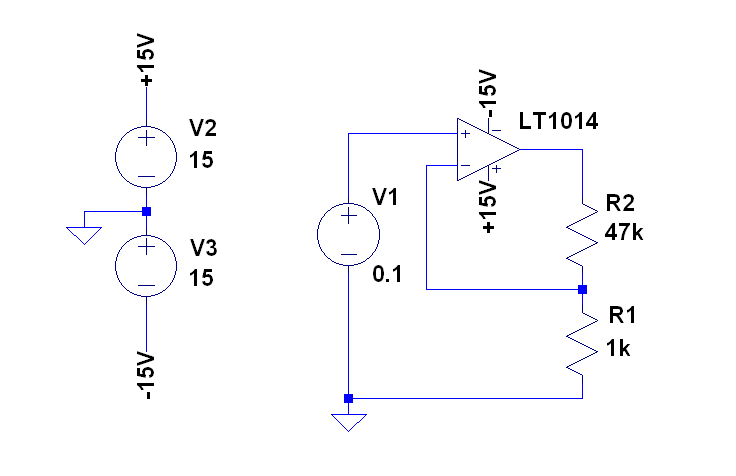
\includegraphics[height=8cm,width=12cm]{Simulationen/OPV}
 \caption{Operationsverstärker beschaltet}
\end{figure}

Die Widerstände wurden im $k\Omega$-Bereich gewählt, um die den Messfehler der Messgeräte möglichst gering zu halten. Die Verstärkung des Operationsverstärker setzt
sich aus dem Verhältniss der beiden Widerstände zusammen, $V_u=1+\frac{47k\Omega}{1k\Omega}=48$, daraus ergeben sich folgende Messwerte.\\

\begin{figure}[H]
 \centering
 \begin{tabular}{c|c}
 $U_e$ 		& $0,1V$ 	\\ \hline
 $U_a$ 		& $4,79V$ 	\\ \hline
 $U_{R1}$ 	& $0,1V$ 	\\ \hline
 $U_{in+}$	& $0,1V$ 	\\ \hline
 $U_{in-}$ 	& $0,99V$ 	\\ \hline
 $I_{R1}$ 	& $0,1mA$ 	\\ \hline
 $I_{R2}$ 	& $0,1mA$ 	\\ \hline
 $I_{in+}$ 	& $0mA$ 	\\ \hline
 $I_{in-}$ 	& $0mA$ 	\\ \hline
 \end{tabular}
 \caption{Simulierte Daten}
\end{figure}

Die Messdaten der Simulation zeigen die zuvor berechnete 48fache Verstärkung der Ausgangsspannung, sowie nahezu keinen Potentialunterschied zwischen den Steuereingängen.
Daher ist auch die Spannung die am Widerstand $R_1$ abgfällt gleich der Eingangsspannung. Die Ströme an den Eingängen des Operationsverstärkers sind gleich $0mA$, da er
sehr hohen Innenwiderstände besitzt. Dadurch fließtauch über beide Widerstände der gleiche Strom. Dies erlaubt es, die Ausgangsspannung über die Spannungsteilerregel zu
berechnen.\\

\begin{align*}
 \frac{U_a}{U_e} &= \frac{R_1 + R_2}{R_1}\\
 U_a &= U_e \left( 1+\frac{R_2}{R_1} \right)\\
\end{align*}

\subsection{Frequenzverhalten}

\begin{figure}[H]
  \centering
  \begin{tikzpicture}
    \begin{axis}[width=15cm, height=10cm, xmin=0, xmax=100e-3, xlabel={t}, ylabel={$U_e$},y tick label style={grid=major}]
      \addplot table[x=time, y=V(n001), mark=none] {csv_files/OPV_Ue_1.csv};
      \addplot table[x=time, y=V(n002), mark=none] {csv_files/OPV_Ua_1.csv};
    \end{axis}
  \end{tikzpicture}
  \caption{symmetrisches Rechtecksignal, $V_{PP}=0.2V, f=100Hz$}
\end{figure}

\begin{figure}[H]
  \centering
  \begin{tikzpicture}
    \begin{axis}[width=15cm, height=10cm, xmin=0, xmax=1e-3, xlabel={t}, ylabel={$U_e$},y tick label style={grid=major}]
      \addplot table[x=time, y=V(n001), mark=none] {csv_files/OPV_Ue_2.csv};
      \addplot table[x=time, y=V(n002), mark=none] {csv_files/OPV_Ua_2.csv};
    \end{axis}
  \end{tikzpicture}
  \caption{symmetrisches Rechtecksignal, $V_{PP}=0.2V, f=10kHz$}
\end{figure}

Der Operationsverstärker besitzt auf Grund seiner Bauweise ein Tiefpassfilter-Verhalten 1.Ordnung. Dies führt dazu, dass die Verstärkung ab einer Grenzfrequenz,
von ca. $1kHz$, mit $20db/DEK$ abnimmt. Bei einer Transitfrequenz von ca. $10MHz$ ist keine Verstärkung mehr vorhanden.\\
Dies kann man gut an den beiden Simulationen erkennen. In der zweiten Simulation kann man erkennen, wie der interne Kondensator bei hohen Frequenzen das Signal
beeinflusst.\\

% !TEX root = deckblatt3a.tex

\section{Invertierender Verst\"arker}
\subsection{Simulationsschaltung}
\begin{figure}[H]
  \begin{center}
    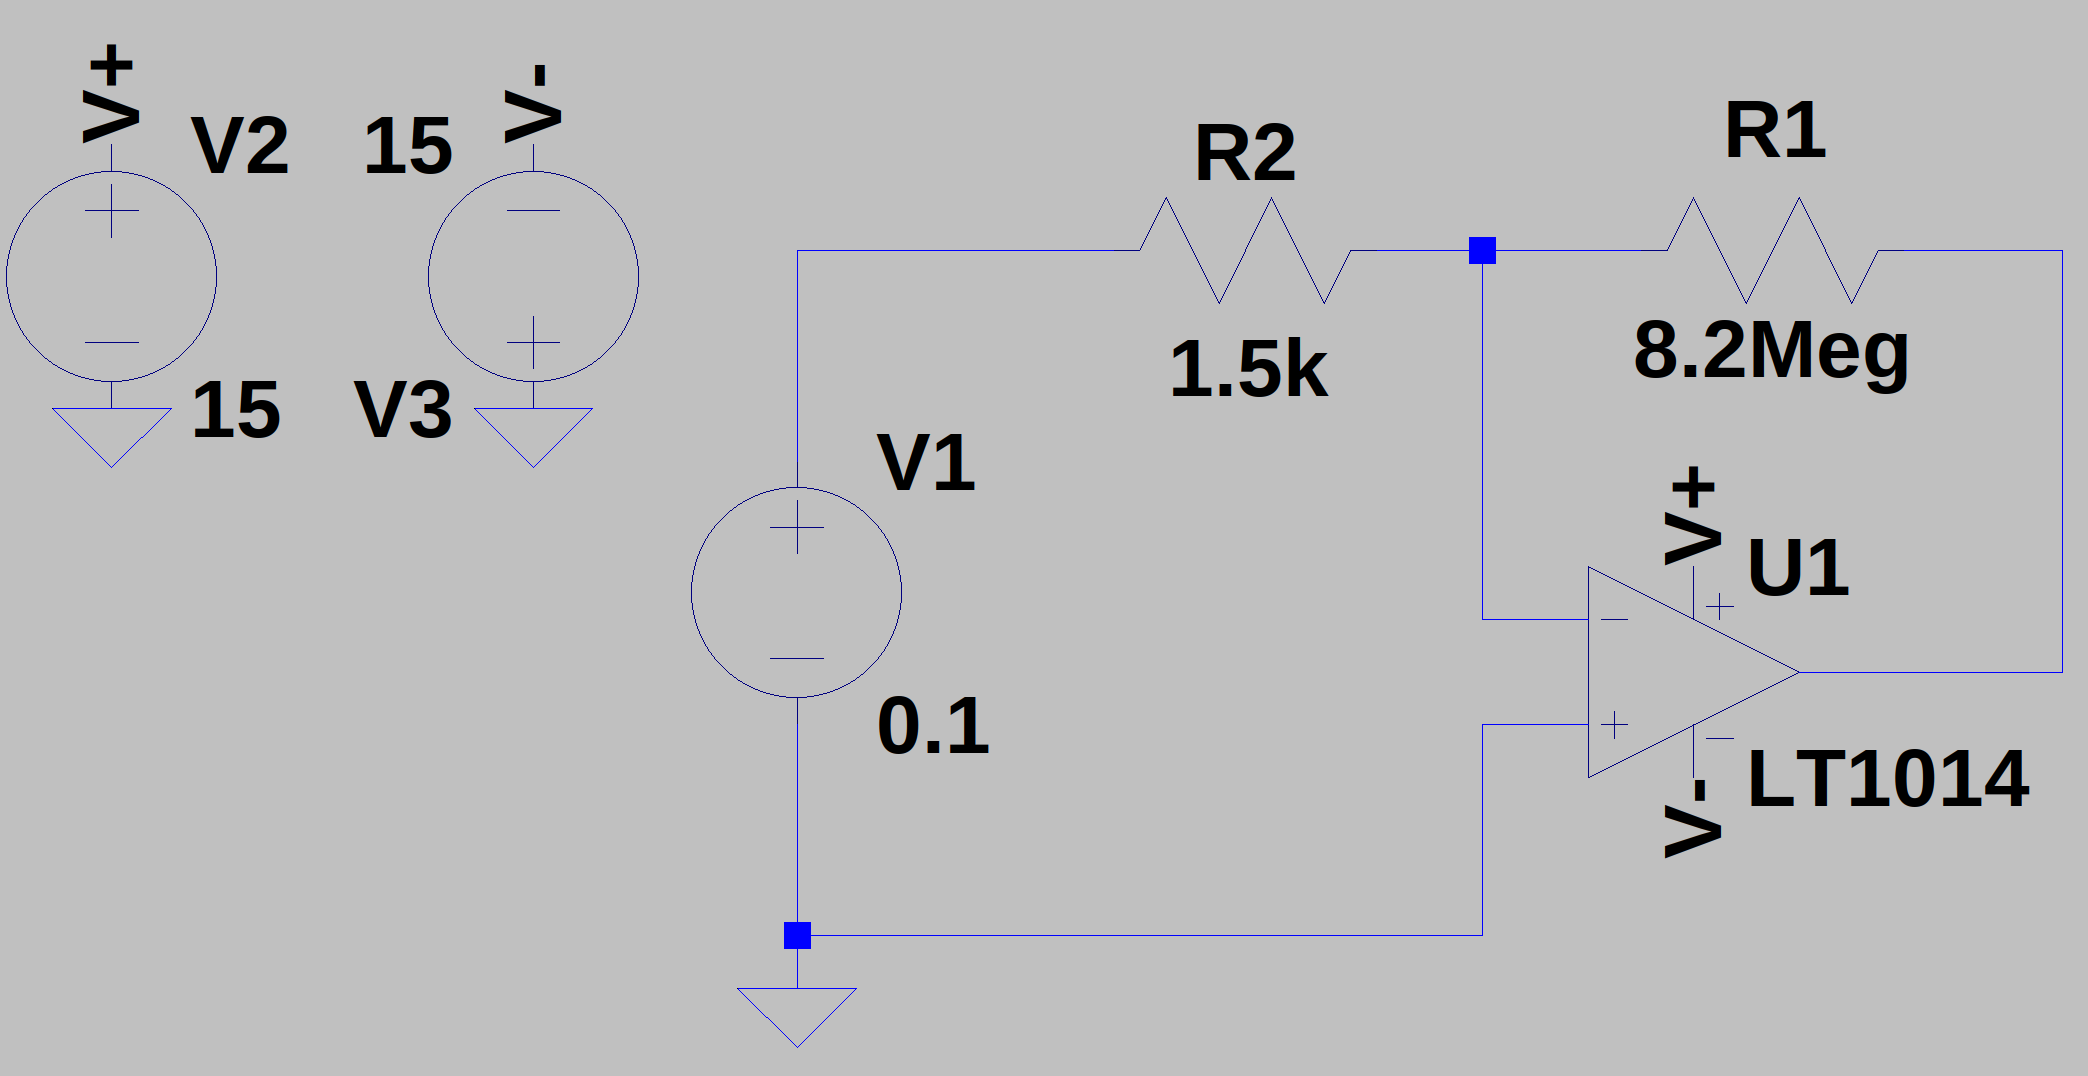
\includegraphics[width=1\textwidth]{./Schaltungen/InvertierenderVerstaerker.png}
    \caption{Simulationsschaltung}
  \end{center}
\end{figure}
\noindent
Da es sich bei dieser Schlatung um einen invertierenden Verst\"arker handel, wird die Eingangsspannung am invertierendne Eingang des OPV geschaltet.
Der Ausgang wird ebenfalls auf den invertierendne Eingang gegengekoppelt umd eine Brauchbare Verst\"arkung einstellen zu k\"onnen. Ein Idealer OPV ohne Gegenkopplung w\"urde die Differenzspannung zwischen invertierenen und nicht-invertierendne Eingang $\infty$ verst\"arken. Die Vert\"arkung wird mit den Beiden Widerst\"anden $R_1$ und $R_2$ eingestellt. Die Beiden Spannungspquellen $V_2$ und $V_3$ stellen die Symetrische Versorgungsspannung von $-15V$ bis $+15V$ dar.\\ \\
$\frac{U_e}{U_a}=-\frac{R_1}{R_2} \Rightarrow U_a=-U_e*\frac{R_2}{R_1} \Rightarrow V=-\frac{R_2}{R_1}$ \\ \\
Da sich die Verst\"arkung $V$ laut Angabe zwichen $-40$ und $-60$ befinden soll wurden f\"ur die Widerst\"ande folgende Werte gew\"ahlt: \\ \\
$R_1=82k\Omega$ \\
$R_2=1,5k\Omega$ \\
$V=-\frac{82k \Omega}{1,5k\Omega}=-54,7$

\subsection{Str\"ome und Spannungen}
Am Eingang des Invertierenden Verst\"arkers wurde wie in der Simulationsschaltung eine Spannungsquelle mit $100mV$ angeschlossen.

\begin{figure}[H]
  \centering
  \begin{tabular}{c|c||c|c}
    $U_e$ & $100mV$ & & \\ \hline
    $U_a$ & $-5,47V$ & & \\ \hline
    $U_{R_1}$ & $-5,47V$ & $I_{R_2}$ & $-66,68\mu A$  \\ \hline
    $U_{R_2}$ & $100mV$ & $I_{R_1}$ & $-66,68\mu A$  \\ \hline
    $U_{IN-}$ & $786nV$ & $I_{IN-}$ & $-12nA$  \\ \hline
    $U_{IN+}$ & $0V$ & $I_{IN+}$ & $0A$
  \end{tabular}
  \caption{Spannungen und Str\"ome}
\end{figure}
\noindent
Die Ausgangsspannung $U_a$ ergibt sich aus $U_e*V$, dies ergibt in diesem Fall $-5,47V$. Der nicht invertierende Eingang ist auf Masse geschaltet, da ein OPV immer Versucht die Spannung an beiden Eing\"angen gleich zu halten, befindet sich am invertierenden Eingang die sogenannte "virtuelle Masse". Daraus folgt wiederum, dass am $R_2$ die $100mV$ Eingangsspannung abfallen und am $R_1$ die $-5,47V$ Ausgangsspannung.
\\ Da der Eingang eines OPV sehr hochohmig ist (ideal: $R_{in}=\infty$) flie\ss{}t auch kein Strom hinein,  daraus folgt wiederum dass die Str\"ome durch $R_1$ und $R_2$ gleich sein m\"ussen.

\subsection{Zeitbereich}
\begin{figure}[H]
  \centering
  \begin{tikzpicture}
    \begin{axis}[width=15cm, height=10cm, xmin=0, xmax=100e-3, xlabel={t}, ylabel={$U[V]$},y tick label style={grid=major}]
      \addplot table[x=time, y=Ue, mark=none] {csv_files/invVer_time1.csv};
      \addplot table[x=time, y=Ua, mark=none] {csv_files/invVer_time1.csv};
    \end{axis}
  \end{tikzpicture}
  \caption{symmetrisches Dreieck, $V_{PP}=0.1V, f=100Hz$}
\end{figure}
\noindent
In dieser Simulation ist ein sch\"ones Verst\"arker Verhalten zu erkennen. Das Eingansignal mit einer Amplitude von $V_{PP} = 100mV$ wird mit der zuvor Errechneten Verst\"arkung von $V=-54,7$ verst\"arkt um am Ausgang des OPVs ausgegeben.

\begin{figure}[H]
  \centering
  \begin{tikzpicture}
    \begin{axis}[width=15cm, height=10cm, xmin=0, xmax=1e-3, xlabel={t}, ylabel={$U[V]$},y tick label style={grid=major}]
      \addplot table[x=time, y=Ue, mark=none] {csv_files/invVer_time2.csv};
      \addplot table[x=time, y=Ua, mark=none] {csv_files/invVer_time2.csv};
    \end{axis}
  \end{tikzpicture}
  \caption{symmetrisches Dreieck, $V_{PP}=0.1V, f=10kHz$}
\end{figure}
\noindent
Ein realer OPV verh\"alt sich intern \"anlich wie ein Tiefpassfilter, je h\"oher die Frequnez desto geringer wird die D\"ampfung. Dies ist in dieser Simulation sehr gut zu erkennen, das Ausgangssignal ist im Vergleich zu der vorherigen Messung stark verschliffen und wird nicht mehr so gut verst\"arkt.


\subsection{Bodediagramme}
\begin{figure}[H]
  \centering
  \begin{tikzpicture}
    \begin{axis}[width=15cm, height=7cm, xmin=1, xmax=100e5, , xmode=log, xlabel={$Hz$}, ylabel={dB},y tick label style={grid=major}]
      \addplot table[x=Frequenz, y=dB,col sep=comma, mark=none] {csv_files/invVer_bode1.csv};
    \end{axis}
  \end{tikzpicture}
  \caption{Amplitudengang, $V=-54,7$}
\end{figure}
\begin{figure}[H]
  \centering
  \begin{tikzpicture}
    \begin{axis}[width=15cm, height=7cm, xmin=1, xmax=100e5, , xmode=log, xlabel={$Hz$}, ylabel={dB},y tick label style={grid=major}]
      \addplot table[x=Frequenz, y=Phase,col sep=comma, mark=none] {csv_files/invVer_bode1.csv};
    \end{axis}
  \end{tikzpicture}
  \caption{Phasengang, $V=-54,7$}
\end{figure}
\noindent
Das zuvor erw\"ahnt Tiefpassverhalten spiegelt sich in diesem Bodediagramm wieder. Ab einer Grenzfrequenz von etwar $20kHz$ wird die Verst\"arkung dieser Schaltung weniger und f\"allt zun\"achst mit $-20dB/Dek$, diese steigt letztlich sogar auf $-40dB/Dek$ an.

\begin{figure}[H]
  \centering
  \begin{tikzpicture}
    \begin{axis}[width=15cm, height=7cm, xmin=1, xmax=100e5, , xmode=log, xlabel={$Hz$}, ylabel={dB},y tick label style={grid=major}]
      \addplot table[x=Frequenz, y=dB,col sep=comma, mark=none] {csv_files/invVer_bode2.csv};
    \end{axis}
  \end{tikzpicture}
  \caption{Amplitudengang, , $V=-5,47$}
\end{figure}
\begin{figure}[H]
  \centering
  \begin{tikzpicture}
    \begin{axis}[width=15cm, height=7cm, xmin=1, xmax=100e5, , xmode=log, xlabel={$Hz$}, ylabel={dB},y tick label style={grid=major}]
      \addplot table[x=Frequenz, y=Phase,col sep=comma, mark=none] {csv_files/invVer_bode2.csv};
    \end{axis}
  \end{tikzpicture}
  \caption{Phasengang, $V=-5,47$}
\end{figure}
\noindent
Bei diesem Bodediagramm wurde die Verst\"arkung von $V=-54,7$ auf $V=-5,47$ verringert, dies erfolte durch eine Veringerung von $R_1$ auf $8,2k\Omega$. Durch das \"Andern der Schaltungseigenschaften verschiebt sich die Grenzfrequenz des OPVs nach hinten. Anstatt bereits bei $20kHz$ beginnt die D\"ampfung bei dieser Schaltung erst eine Dekade sp\"ater bei etwar $200kHz$. Daraus l\"asst sich folgern, dass die Verst\"arkung der OPV Schaltung mit der Grenzfrequenz direkt proportional zusammenh\"angt.

% !TEX root = deckblatt2b.tex

\section{Integrierer}

\begin{figure}[H]
 \centering
 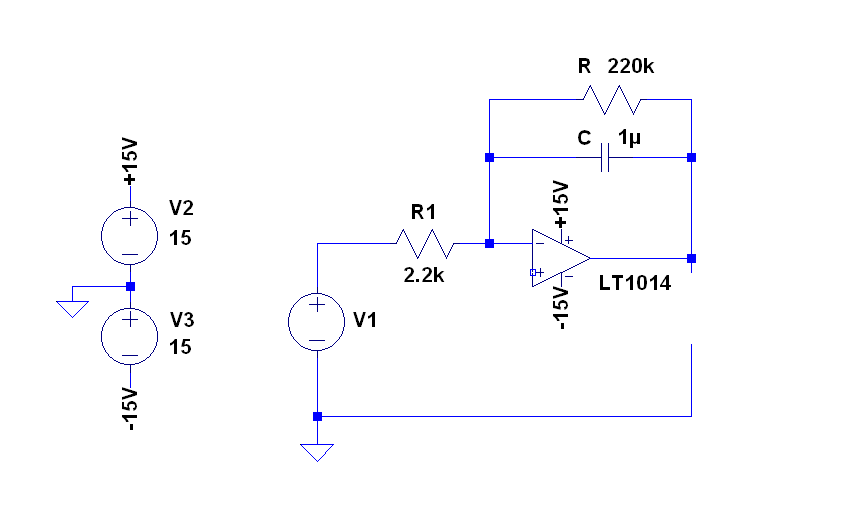
\includegraphics[height=8cm,width=12cm]{Simulationen/Integrator}
 \caption{Operationsverstärker als Integrator beschaltet}
\end{figure}
\noindent
In dieser Beschaltung gibt die Ausgangsspannung das Integral der Eingangsspannung über die Zeit an. Der Widerstand $R$ dient nur zur stabilisation
der Schaltung und wird daher vernachlässigt, er sollte jedoch wesentlich größer als $R_1$ gewählt werden.

\subsection{Übertragungsfunktion}

Der invertierende Integrierer ist vom Aufbau ähnlich dem invertierenden Verstärker, jedoch wird die Ausgangsspannung hier durch die Spannung am Kondensator beschrieben.\\
\begin{align*}
 U_C &= \frac{1}{C} \int i_c(t)\ \mathrm{d}t\\
 i_c &= I_{R1}\\
 U_C &= \frac{1}{RC} \int U_e(t)\ \mathrm{d}t\\
 U_a &= -U_C\\
\end{align*}
\noindent
Aus dieser Berechnung ergibt sich für das Eingangssignal, in Form einer Rechteckspannung mit fallender Flanke, eine Dreiecksspannung mit steigender Flanke.\\
\begin{align*}
 RC &= 2,2ms\\
 U_e(t) &= 
  \begin{cases}
   \ -\frac{1}{10}\ &0 \leq t < 100ms\\
   \quad \frac{1}{10}\ &100ms < t \leq 200ms\\ 
  \end{cases}
  \quad
  U_a(t) = 
  \begin{cases}
   \quad \frac{t}{22}\ &0 \leq t < 100ms\\
   \ -\frac{t}{22}\ &100ms < t \leq 200ms\\ 
  \end{cases}
\end{align*}

Dieses Ergebnis kann man, nach dem Einschwingvorgang, auch in der Simulation beobachten.\\

\begin{figure}[H]
  \centering
  \begin{tikzpicture}
    \begin{axis}[width=15cm, height=10cm, xmin=0, xmax=2, xlabel={t}, ylabel={$U_e$},y tick label style={grid=major}]
      \addplot table[x=time, y=V(n003), mark=none] {csv_files/Integrator_Ue.csv};
      \addplot table[x=time, y=V(n002), mark=none] {csv_files/Integrator_Ua.csv};
    \end{axis}
  \end{tikzpicture}
  \caption{$U_e$ symmetrisches Recktecksignal, $V_{PP}=0.2V, f=5Hz$}
\end{figure}

\subsection{Bode-Diagramm}

\begin{figure}[H]
  \centering
  \begin{tikzpicture}
    \begin{axis}[width=15cm, height=7cm, xmin=1, xmax=100e3, , xmode=log, xlabel={$Hz$}, ylabel={dB},y tick label style={grid=major}]
      \addplot table[x=Freq, y=V(n002),col sep=comma, mark=none] {csv_files/Integrator_dB.csv};
      %\addplot table[x=Freq, y=Phi,col sep=comma, mark=none] {csv_files/Integrator_Phi.csv};
    \end{axis}
  \end{tikzpicture}
  \caption{Frequenzgang}
\end{figure}
\begin{figure}[H]
  \centering
  \begin{tikzpicture}
    \begin{axis}[width=15cm, height=7cm, xmin=1, xmax=100e3, , xmode=log, xlabel={$Hz$}, ylabel={dB},y tick label style={grid=major}]
      %\addplot table[x=Freq, y=V(n002),col sep=comma, mark=none] {csv_files/Integrator_dB.csv};
      \addplot table[x=Freq, y=Phi,col sep=comma, mark=none] {csv_files/Integrator_Phi.csv};
    \end{axis}
  \end{tikzpicture}
  \caption{Phasengang}
\end{figure}

Das Bode-Diagramm zeigt die Abnahme der Verstärkung bei steigender Frequenz, mit $20dB/DEK$. Die Transitfrequenz liegt bei dieser OPV-Schaltung
bei ca. $30Hz$, danach wirkt er dämpfend.\\

% !TEX root = deckblatt3a.tex

\section{Invertierender Schmitt-Trigger}
\subsection{Simulationsschaltung}
\begin{figure}[H]
  \begin{center}
    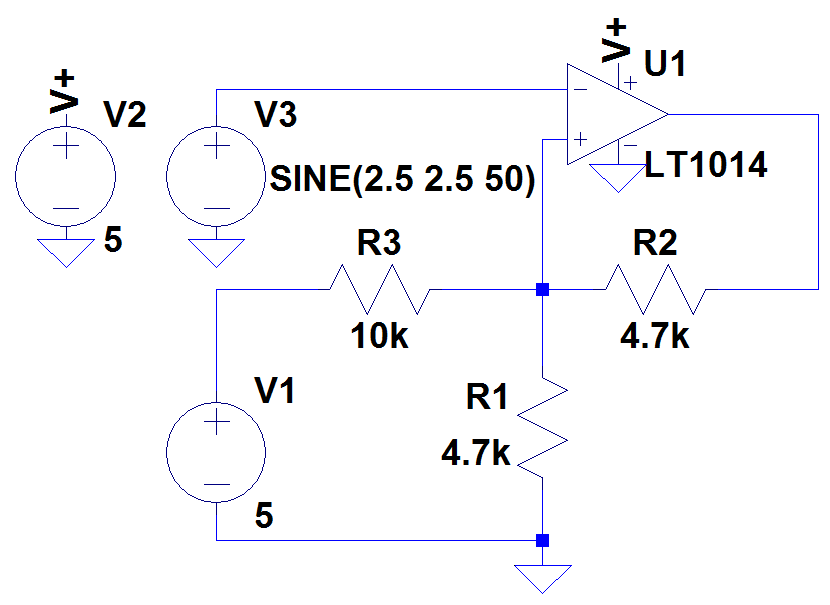
\includegraphics[width=1\textwidth]{./Schaltungen/InvertierenderSchmittTrigger.png}
    \caption{Simulationsschaltung}
  \end{center}
\end{figure}
\noindent
Da das Eingangsignal an den invertierenden Eingang geschaltet ist, ist diese OPV Schaltung auf jeden Fall invertierend. Die Ausgangsspannung wird auf den nicht-invertierenden Eingang r\"uckgekoppelt, das hei\ss{}t es handelt sich um eine Mittkopplung, das hei\ss{}t der OPV wird bei jedem Eingangssignal entweder nach oben oder nach unten \"ubersteuern.

\subsection{Berechnung Superpositionsprizip}
$U_{high}=4,39V$ \\
$U_{low}=0,029V$ \\ \\
$R_{12}=2,35k\Omega$ \\
$R_{13}=3,19k\Omega$ \\ \\
\begin{itemize}
  \item \textbf{1. Fall: $U_{high}$} \\ \\
        \textbf{Kurzgeschlossen: $U_a$ }\\
        $U_{p1} = U_{VCC}*\frac{R_{12}}{R_{12}+R_3} = 5V * \frac{2,35}{12,35} = 0,951V$ \\ \\
        \textbf{Kurzgeschlossen $U_{VCC}$}\\
        $U_{p2} = U_{VCC}*\frac{R_{13}}{R_{13}+R_2} = 4,39V * \frac{3,19}{7,90} = 1,777VV$ \\ \\
        $\Rightarrow U_p = U_{p1} + U_{p1} = 2,728V$

  \item \textbf{2. Fall: $U_{low}$} \\ \\
        \textbf{Kurzgeschlossen: $U_a$ }\\
        $U_{p1} = U_{VCC}*\frac{R_{12}}{R_{12}+R_3} = 5V * \frac{2,35}{12,35} = 0,951V$ \\ \\
        \textbf{Kurzgeschlossen $U_{VCC}$}\\
        $U_{p2} = U_{VCC}*\frac{R_{13}}{R_{13}+R_2} = 0,029V * \frac{3,19}{7,90} = 0,0117V$ \\ \\
        $\Rightarrow U_p = U_{p1} + U_{p1} = 0,963V$
\end{itemize}


\subsection{Simulationen}
\begin{figure}[H]
  \centering
  \begin{tikzpicture}
    \begin{axis}[width=15cm, height=10cm, xmin=0, xmax=100e-3, xlabel={t}, ylabel={$U[V]$},y tick label style={grid=major}]
      \addplot table[x=time, y=V(n001), mark=none] {csv_files/invSchmitt_time1.csv};
      \addplot table[x=time, y=V(n002), mark=none] {csv_files/invSchmitt_time1.csv};
      \addplot table[x=time, y=V(n003), mark=none] {csv_files/invSchmitt_time1.csv};
    \end{axis}
  \end{tikzpicture}
  \caption{Sinus, $V_{PP}=5V, f=50Hz$,}
\end{figure}
\noindent
In dieser Abbildung ist die Eingangsspannung(blau), die Ausgangsspannung(rot) und die Schaltung am nicht-invertierenden Eingang(braun) des OPVs zu sehen. Mit den drei Widerst\"anden und der Referenzspannung von $5V$ werden die Schaltschwellen eingestellt. Die obigen Berechnungen werden in diesem Diagramm best\"atigt da man die Schaltschwellen von $0,963V$ bzw. $2,729V$ sehr gut erkennen kann. \\
Erreicht der Sinus $2,729V$ auf der steigenden Flanke springt der Ausgnag auf $-U_v$ in diesem Fall Masse, und werden $0,963V$ auf der fallenden Flanke erreicht springt der Ausgang auf $+U_v$ in diesem Fall $5V$. Der Wert der positiven Versorgungsspannung wird nicht genau erreicht da es sich nicht um einen 'Rail-to-Rail' OPV handelt.

\begin{figure}[H]
  \centering
  \begin{tikzpicture}
    \begin{axis}[width=15cm, height=10cm, xmin=0, xmax=1e-6, xlabel={t}, ylabel={$U[V]$},y tick label style={grid=major}]
      \addplot table[x=time, y=V(n001), mark=none] {csv_files/invSchmitt_time2.csv};
      \addplot table[x=time, y=V(n002), mark=none] {csv_files/invSchmitt_time2.csv};
      \addplot table[x=time, y=V(n003), mark=none] {csv_files/invSchmitt_time2.csv};
    \end{axis}
  \end{tikzpicture}
  \caption{Dreieck, $V_{PP}=5V, f=5MHz$}
\end{figure}
\noindent
Wie in der Abbildung zu erkennen ist, ist die Spannung am Ausgang bzw. am nicht-invertierenden Eingang des OPVs konstant. Dies liegt daran, dass ein realer OPV nicht unendlich schnell schalten kann. Eine Frequnezn von $5MHz$ ist f\"ur diesen OPV definitief zu schnell und am Ausgang wird nun etwas f\"ollig anderes Ausgegeben als man es sich von einem Schmitt-Trigger erwarten w\"urde.


\end{document}
